\chapter{Planificación y metodología}

En este capítulo se procederá a explicar la metodología diseñada para el proyecto. Esta se ideó para ajustarse a las necesidades, retos y riesgos del desarrollo de videojuegos que se identificaron en el capítulo del estado del arte. Tras ello, se procederá al apartado de planificación, en el que se detallará la programación temporal inicial. Por último, en el apartado de seguimiento, se detallará el desarrollo de las distintas fases y sprints, además de realizar una retrospectiva comparando el desarrollo con la planificación inicial.

\section{Metodología}

En el capítulo anterior se detectaron una serie de riesgos y problemas comunes en el desarrollo de videojuegos, que se recapitulan a continuación:

\begin{itemize}
    \item \textbf{Alcance del proyecto y \textit{feature creep}}, la adición descontrolada de contenido por planificación pobre.
    \item \textbf{Integración de recursos multimedia} como arte o sonido.
    \item \textbf{Convivencia del proceso creativo con el de ingeniería}, tanto de las distintas disciplinas asociadas como de la construcción del propio videojuego.
    \item \textbf{Búsqueda del \textit{fun factor}}.
    \item Gestión de proyectos con plantillas de empleados grandes y diversas.
    \item \textbf{Satisfacción del público objetivo del juego}, calibrar la experiencia para que esté al nivel de dificultad esperado.
    \item \textbf{Uso de crunch}, o agotar el presupuesto del proyecto.
\end{itemize}

Se diseñó la metodología con el objetivo de tratar los puntos en negrita de la anterior lista. Al ser un proyecto individual, no se puede gestionar el aspecto de gestión de proyecto multidisciplinar 

El desarrollo contará con 4 fases: \textbf{preproducción, producción, postproducción} y \textbf{despliegue}.

\subsection{Preproducción}

\begin{figure}[H]
    \centering
    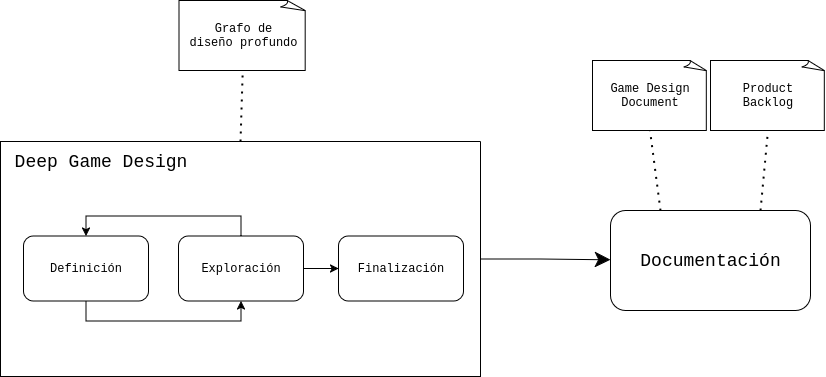
\includegraphics[scale=0.50]{img/preproduction.drawio.png}
    \caption[Diagrama de preproducción]{Diagrama del proceso de preproducción.}
    \label{fig:preproduction}
\end{figure}

La preproducción comienza aplicando \textbf{Deep Game Design}\cite{deepdesign}. Se experimentará con prototipos rápidos y baratos las ideas de diseño sobre las que se cimentará el juego. Se plantearán y verificarán las distintas restricciones (es decir, las mecánicas y reglas del juego) y los diferentes puzles (desafíos) que se le plantearán al jugador. En esta fase se producirá el \textit{diagrama de diseño profundo}, con sus métricas de profundidad, complejidad y elegancia. Una vez finalizada esta fase, se tendrá una comprensión profunda de las mecánicas principales alrededor de las que se construirá el juego.

Con este conocimiento adquirido se pasará a desarrollar una primera iteración del \textit{Game Design Document} (GDD), donde se desarrollará el \textit{pitch} (concepto) del juego, su contexto, narrativa, mecánicas principales, estílo artístico, estructura general del juego, etc. Este documento podrá ser modificado en etapas posteriores.

A continuación se redactará el \textit{product backlog}. Esto es un artefacto de SCRUM, ya que en producción se trabajará con una versión adaptada de esta metodología. Se trata de una lista ordenada de requisitos del proyecto, normalmente en forma de historias de usuario.

Las \textbf{historias de usuario} son requisitos formalizados desde la perspectiva del usuario. Suelen tener la misma estructura:\\ 


\centerline{\textit{Como [tipo de usuario] quiero hacer [actividad] para [objetivo]}}

Por ejemplo: \textit{''como usuario, quiero poder revisar la foto que acabo de hacer con la cámara de mi móvil para comprobar si he salido bien''}. Este formato es ideal para expresar requisitos funcionales. Se realiza desde la perspectiva del usuario expresando una necesidad suya, y no una solución de implementación concreta. En este proyecto se emplearía para cuestiones como funciones de guardado, de accesibilidad o de ajustes de usuario. Sin embargo, como se ha comentado anteriormente, no se puede expresar el núcleo jugable del juego, su estética o su \textit{fun factor} con la estructura de una historia de usuario. Para ello se propone el siguiente artefacto: \textbf{historia de juego}.

Las historias de juego son una formalización de las ideas plasmadas en el \textit{GDD}. Su objetivo es representar el requisitado más emocional y abstracto del proyecto y poder añadirlo al \textit{product backlog}. Siguen la siguiente estructura:\\

\centerline{\textit{El [actividad/elemento] es [adjetivo]}}

Por ejemplo, \textit{es divertido rebotar en los enemigos}, \textit{es divertido recolectar monedas}, \textit{el cansancio del personaje transmite la dureza de subir una montaña}, o \textit{los entornos transmiten nostalgia}. Las historias de juego son un artefacto \textbf{exclusivamente representativo} de los requisitos emocionales del juego dentro del product backlog, siendo responsabilidad del \textit{GDD} explicarlos y contextualizarlos. Se propone hacer esto así para tenerlos como elementos operables durante los \textit{sprints} de producción y poder visualizarlos en los \textit{tableros kanban} que se realizarán en la misma.

Por último, se realizará una estimación del proyecto con un presupuesto en forma de horas efectivass de trabajo. El desarrollo completo hasta la salida del juego no deberá sobrepasar este número.

\subsection{Producción}

\begin{figure}[H]
    \centering
    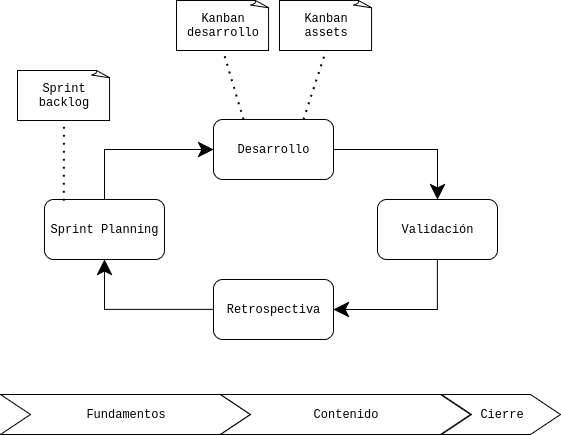
\includegraphics[scale=0.50]{img/production.drawio.png}
    \caption[Diagrama de produccion]{Diagrama del proceso de producción.}
    \label{fig:production}
\end{figure}


Para la producción se usará una versión adaptada de SCRUM. Estará dividida en \textit{sprints} de alrededor de 20 horas de trabajo efectivo. Los sprints son iteraciones del proyecto con un tiempo fijo. Tienen la siguiente estructura:

\begin{itemize}
    \item \textbf{\textit{Sprint planning}}: Se revisa el product backlog, se escogen las historias de usuario que se desarrollarán en ese sprint y se derivan tareas relacionadas con estas a el \textit{sprint backlog}. Para cada tarea se realiza una estimación en horas para su compleción y qué \textit{assets} se requieren.
    \item \textbf{Desarrollo}: Se hace uso de un \textit{tablero kanban} para gestionar el estado de las diferentes tareas, el cual puedes ser diseño, implementación, validación, test, finalizado y descartado. Se tiene otro tablero kanban para llevar la cuenta y el progreso de la producción de los distintos assets. En este punto se desarrollan los test automáticos asociados 
    \item \textbf{Validación}: Una vez finalizado el grueso del sprint, se realiza una sesión íntegra del producto resultante. Durante esta se realizan anotaciones sobre la experiencia percibida, las sensaciones, qué elementos funcionan a nivel emocional y cuales no. Si se detecta algún problema en esa línea, se anotará en el product backlog en forma de \textbf{observación de test}. Esta es un tipo de entrada al mismo nivel que las historias de usuario o juego. En el se describe el problema detectado en el juego, para el cual deberá diseñarse una solución en sprints posteriores.
    \item \textbf{Retrospectiva}: Se realiza un repaso del desempeño del sprint, redactando en un pequeño documento qué se ha hecho bien, qué se ha hecho mal, qué imprevistos han surgido y cómo se adaptará el proyecto en siguientes sprints. Por último se hace una primera aproximación sobre qué parte del product backlog se tratará en el siguiente sprint.
\end{itemize}

A su vez, los sprints de producción se encasillan en tres etapas sucesivas:

\begin{itemize}
    \item \textbf{Fundamentos} (40\% del total): En esta se desarrolla el núcleo jugable y funcional del juego. Esto abarca asuntos como el bucle principal de ejecución, el desarrollo completo del personaje principal y herramientas que faciliten la creación de contenido para el proyecto, como un constructor de mapas, plantillas para implementar enemigos, un sistema de diálogos, el sistema de cámaras, etc. Es especialmente importante verificar la calidad del núcleo jugable, ya que este a penas será modificado más adelante.
    \item \textbf{Contenido} (40\% del total): Usando las herramientas de la fase anterior, se añade contenido al juego de manera iterativa: más enemigos, más escenarios, o mecánicas concretas. Por ejemplo, si se desarrolla una zona de volcanes, se implementa una mecánica a través de la cual el personaje puede quemarse con la lava. Estas mecánicas por su naturaleza puntual, deben ser más simples y sencillas de implementar que el núcleo del juego.
    \item \textbf{Cierre} (20\% del total): Se cesa de añadir contenido nuevo con el objetivo de cerrar la experiencia con lo que ya se tiene hecho. Al final de esta fase, la producción acaba y el juego debe ser jugable de principio a fin.
\end{itemize}

Durante la fase de contenidos se producirá una versión de prueba del juego. Se empleará en una prueba con usuarios reales, con el objetivo de obtener retroalimentación sobre el juego, ver qué aspectos gustan, cuales no y poder reaccionar con tiempo para aplicar cambios en la planificación de ser necesario.

\subsection{Postproducción}

\begin{figure}[H]
    \centering
    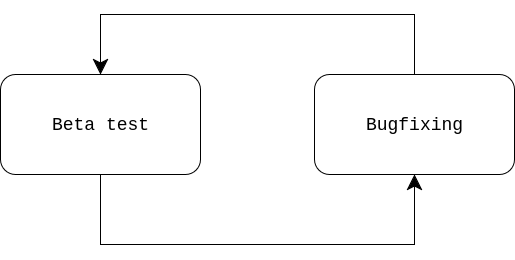
\includegraphics[scale=0.50]{img/postproduction.drawio.png}
    \caption[Diagrama de postproducción]{Diagrama del proceso de postproducción.}
    \label{fig:postproduction}
\end{figure}

Durante la postproducción se produce una fase intensiva de test para detectar y corregir bugs. Se prueba el juego por usuarios, tanto de dentro del equipo de desarrollo como fuera de él, en sesiones monitorizadas siempre que sea posible. Además de solventar bugs se realizan cambios estéticos para pulir el apartado visual. Se hace uso de un tablero kanban donde se anotan todos los bugs y problemas derivados de las sesiones de test.

\subsection{Despliegue}

\begin{figure}[H]
    \centering
    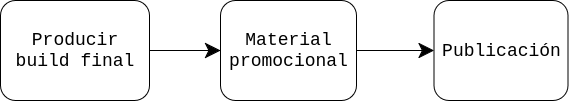
\includegraphics[scale=0.50]{img/deploy.drawio.png}
    \caption[Diagrama de despliegue]{Diagrama del proceso de despliegue.}
    \label{fig:deploy}
\end{figure}

Se compila el juego y se prepara para su publicación por el medio correspondiente (Steam, \textit{itch.io}, consolas, etc.). También se preparan materiales promocionales como un trailer y recursos gráficos.

\section{Planificación}

\section{Seguimiento}

